% Appendix B

\appendix
\renewcommand{\thechapter}{B}
\chapter{Paquete kcorebip, manual de uso} % Main appendix title

\label{APP_KCOREMANBIP} % For referencing this appendix elsewhere, use \ref{AppendixA}

\section*{Introducción}

El paquete \texttt{kcorebip} realiza la descomposición \texttt{k-core} de una red y su análisis y permite dibujar los diagramas \textit{polar}
y \textit{zigurat}. Funciona para cualquier tipo de red bipartita aunque en lo que sigue se utilizará la terminología de las redes mutualistas.

Se instala desde \texttt{github} usando el comando \texttt{install\_github}$("$\path{jgalgarra/kcorebip}$")$, para lo cual previamente se tiene que cargar el paquete \texttt{devtools}.
 
\subsection*{Formato del fichero de entrada}
\label{input_file_format}

En \texttt{kcorebip} se utiliza el formato de fichero de entrada de la base de datos \href{http://www.web-of-life.es/}{web of life} \cite{bascompte2009}. Los datos se alamacenan en ficheros \texttt{.csv}. Las especies de la clase \textit{a} se distribuyen por columnas y las de nodos \textit{b} por fileas. La primera columna contiene las etiquetas de las especies de la clase b, y la primera fila, las etiquetas de la clase a. Si la matriz de adyacencia es binaria, la celda $especie\_a\_m,especie\_b\_n$ estará rellena con $1$ si hay enlace y con $0$ si no lo hay. Si es pesada, con un numero real diferente de $0$ en el caso de que las especies interactúen.

La norma para nombrar los ficheros es $M\_XX\_NNN.csv$ donde $XX$ es el tipo, $PL$ para redes de polinizadores y $SD$ para dispersores, y $NNN$ un número de serie. No obstante, los ficheros pueden tener el nombre que se desee.

\begin{figure}[h!]
\centering
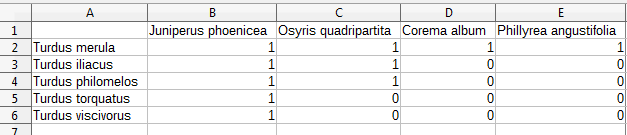
\includegraphics[scale=0.8]{ManFigs/SD_029_csv.png}
\caption {Ejemplo de fichero de entrada, red de dispersores número $029$ de la \href{http://www.web-of-life.es/}{web of life}.}
\label{fig:AKMAN_red_example}
\end{figure}

\subsection*{Análisis de la red}
\label{network_analysis}

La función \texttt{analyze\_network} lleva a cabo la descomposición \textit{k-core}.

\fontsize{3.5mm}{3.5mm}\selectfont
\begin{verbatim}
analyze_network(namenetwork, directory = "", guild_a = "pl",
                guild_b = "pol", plot_graphs = FALSE, only_NODF = FALSE)
\end{verbatim}
\normalsize

Argumentos:
\small
\begin{itemize}

\item \texttt{namenetwork}: nombre del fichero de la matriz de adyacencia.
	
\item \texttt{directory}: directorio en el que se encuentra el fichero de la matriz.

\item \texttt{guild\_a}: prefijo para los nodos almacenadoa en las filas.

\item \texttt{guild\_b}: prefijo para los nodos almacenadoa en las columnas.

\item \texttt{plot\_graphs}: represeantar el histograma de \textit{k-shells} y un gráfico Kamada Kawai.

\item \texttt{only\_NODF}: cacular sólo la medida de anidamiento $NODF$.

\end{itemize}

La función devuelve:
\begin{itemize}
\item \texttt{calc\_values}, una lista que contiene los sigiuentes objetos:
   \begin{itemize}
   
\item \texttt{graph}: la red descrita como un objeto del tipo \texttt{igraph::graph}.

\item \texttt{max\_core}: máxima \texttt{k-shell}

\item \texttt{nested\_values}: una lista de valores de retorno de la función \texttt{bipartite::nested}, salvo que se indique que \texttt{only\_NODF} es TRUE.

\item \texttt{num\_guild\_a}: número de nodos de la clase a.

\item \texttt{num\_guild\_b}: número de nodos de la clase b.

\item \texttt{links}: número de enlaces.

\item \texttt{meandist}: $\overline {k}_{radius}$.

\item \texttt{meankdegree}:  $\overline {k}_{degree}$.

\item \texttt{spaths\_mat}: matriz con los caminos más cortos nodo a nodo.

\item \texttt{matrix}: matriz de adyacencia.

\item \texttt{g\_cores}: lista con los valores de \textit{k-shell} de cada nodo.

\item \texttt{modularity\_measure}: valor de retorno de la función \texttt{igraph::modularity}.
   \end{itemize}


\end{itemize}

\subsection*{Diagrama polar}
\label{polar_plot}

La función \texttt{polar\_graph} permite representar el diagrama polar de una red. La sintaxis de llamada es:

\fontsize{3.5mm}{3.5mm}\selectfont
\begin{verbatim}
polar_graph <- function( red, directorystr = "data/", 
                         plotsdir = "plot_results/polar/", 
                         print_to_file = FALSE, pshowtext = FALSE,
                         show_histograms = TRUE, 
                         glabels = c("Plant", "Pollinator"),
                         gshortened = c("pl","pol"),
                         lsize_title = 22, lsize_axis = 12, 
                         lsize_legend = 13, lsize_axis_title = 14, 
                         lsize_legend_title = 15, file_name_append = "",
                         print_title = TRUE,
                         progress = NULL, printable_labels = 0)
\end{verbatim}
\normalsize

Los parámetros \texttt{red}, \texttt{directorystr} y \texttt{plotsdir} son el nombre de la matriz de adyacencia, el directorio en el que se encuentra y el directorio de salida. Si \texttt{print\_to\_file} es \texttt{FALSE} el diagrama se representa en ventana de la sesión \texttt{R} desde la que se lanza el comando. El nombre del fichero de salida es el del fichero de entrada al que se añade \texttt{\_polar.png}. Los paths son relativos al directorio de trabajo de la sesión \texttt{R} pero también pueden especificarse paths absolutos.

Los ficheros de salida tienen una resolución de 600 dpi y un tamaño de 12 x 12 pulgadas. Si el gráfico se presenta en la ventana de la sesión, los tamaños de las etqiuetas pueden variar en función de las fuentes instaladas y del tamaño de la ventana.

El siguiente comnando crea el fichero \texttt{M\_PL\_001\_polar.png} en el directorio \texttt{grafresults/}

\fontsize{3.5mm}{3.5mm}\selectfont
\begin{verbatim}
polar_graph("M_PL_034.csv","data/",plotsdir="grafresults/",
            print_to_file = TRUE)
\end{verbatim}
\normalsize

\begin{figure}[h!]
\centering
\includegraphics[scale=0.41]{ManFigs/M_PL_034_polar.png}
\caption {Ejemplo de diagrama polar.}
\label{fig:AKMAN_M_PL_034_polar}
\end{figure}

El título del diagrama incluye $\overline{k}_{radius}$, $\overline {k}_{degree}$, $NODF$ \cite{almeida2008consistent} y $Modularity$ usando el método \textit{QanBiMo} \cite{dormann2014method}.

Por defecto, los nodos aparecen sin etiquetas. Se puede elegir que aparezcan algunas con el parámetro \texttt{printable\_labels}. Por ejemplo, si se fija a $3$ se incluirán las de los tres nodos con menor ${k}_{radius}$ y las de los tres con mayor ${k}_{radius}$. Los textos siempre oscurecen el resultado final por lo que habrá que evitarlos en lo posible. Las etiquetas de las clases son configurables, así como las abreviaturas. Esto permite tratar cualquier tipo de red bipartita. La función utiliza de manera automática \texttt{"Plant, Pollinator"} y \texttt{"Plant, Disperser"} si el fichero de entrada sigue la norma de nombrado de \texttt{web of life} pero pueden modificarse con el parámetro de entrada \texttt{glabels}. Tres histogramas se representan bajo el diagrama principal con las distribuciones de $k_{radius}$, $k_{degree}$ y $k_{shell}$. 

La configuración del diagrama polar es muy simple. El siguiente ejemplo muestra como cambiar el aspecto de la figura \ref{fig:AKMAN_M_PL_034_polar}.

\clearpage
\begin{figure}[h!]
\centering
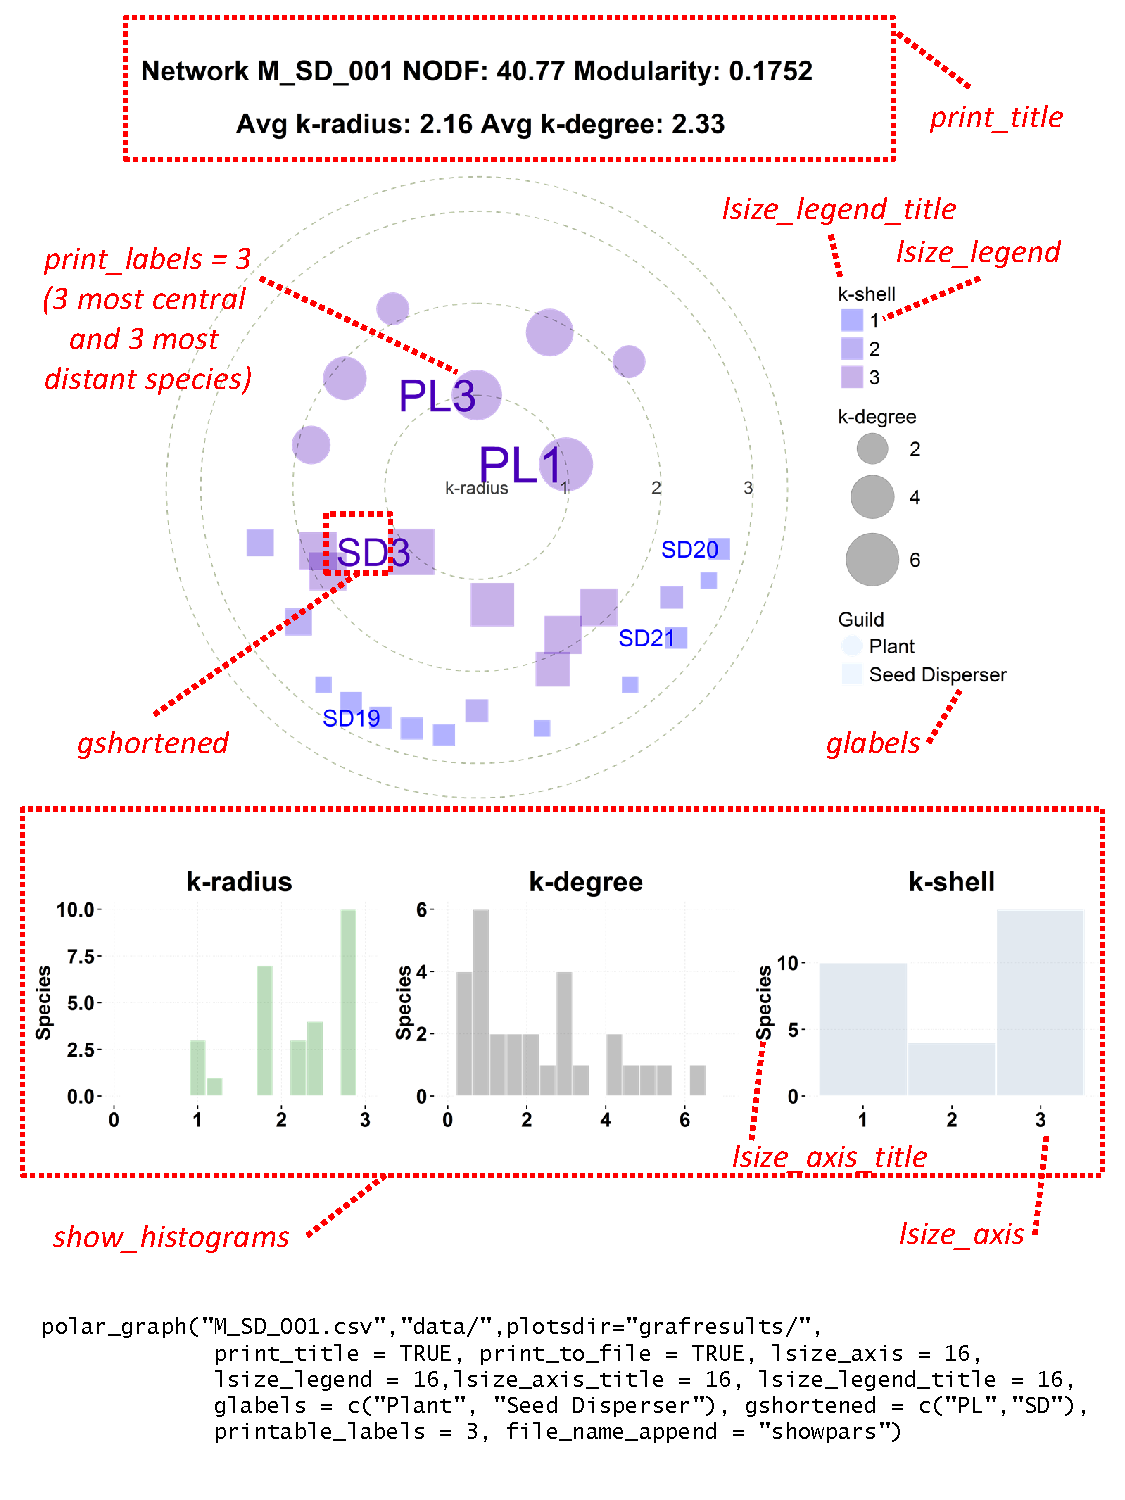
\includegraphics[scale=0.8]{ManFigs/polar_params.pdf}
\caption {Diagrama polar con diversos parámetros de visualización.}
\label{fig:AKMAN_polar_params}
\end{figure}

\clearpage
\subsection*{El diagrama zigurat}

\noindent La función \texttt{ziggurat\_graph} crea el diagrama zigurat de una red bipartita. La sintaxis de llamada es:

\fontsize{3.5mm}{3.5mm}\selectfont
\begin{verbatim}
ziggurat_graph(datadir, filename, paintlinks = TRUE,
	  displaylabelszig = TRUE, print_to_file = FALSE,
	  plotsdir = "plot_results/ziggurat/", flip_results = FALSE,
	  aspect_ratio = 1, alpha_level = 0.2, color_guild_a = c("#4169E1",
	  "#00008B"), color_guild_b = c("#F08080", "#FF0000"),
	  color_link = "slategray3", alpha_link = 0.5, size_link = 0.5,
	  displace_y_b = rep(0, 11), displace_y_a = rep(0, 11), 
	  labels_size = 3.5, lsize_kcoremax = 3.5, lsize_zig = 3, 
	  lsize_kcore1 = 2.5, lsize_legend = 4, lsize_core_box = 2.5, 
	  labels_color = c(), height_box_y_expand = 1, 
	  kcore2tail_vertical_separation = 1, kcore1tail_disttocore = c(1, 1), 
	  innertail_vertical_separation = 1,
	  horiz_kcoremax_tails_expand = 1, factor_hop_x = 1,
	  displace_legend = c(0, 0), fattailjumphoriz = c(1, 1),
	  fattailjumpvert = c(1, 1), coremax_triangle_height_factor = 1,
	  coremax_triangle_width_factor = 1, paint_outsiders = TRUE,
	  displace_outside_component = c(1, 1), outsiders_separation_expand = 1,
	  outsiders_legend_expand = 1,
	  weirdskcore2_horizontal_dist_rootleaf_expand = 1,
	  weirdskcore2_vertical_dist_rootleaf_expand = 0,
	  weirds_boxes_separation_count = 1, root_weird_expand = c(1, 1),
	  hide_plot_border = TRUE, rescale_plot_area = c(1, 1),
	  kcore1weirds_leafs_vertical_separation = 1, corebox_border_size = 0.2,
	  kcore_species_name_display = c(), kcore_species_name_break = c(),
	  shorten_species_name = 0, label_strguilda = "", label_strguildb = "",
	  landscape_plot = TRUE, backg_color = "white", show_title = TRUE,
	  use_spline = TRUE, spline_points = 100, file_name_append = "",
	  svg_scale_factor = 10, progress = NULL)
\end{verbatim}
\normalsize

La configuración del diagrama zigurat es mucho más rica y compleja que la del diagrama polar. 
%
%\begin{figure}[hp!]
%\centering
%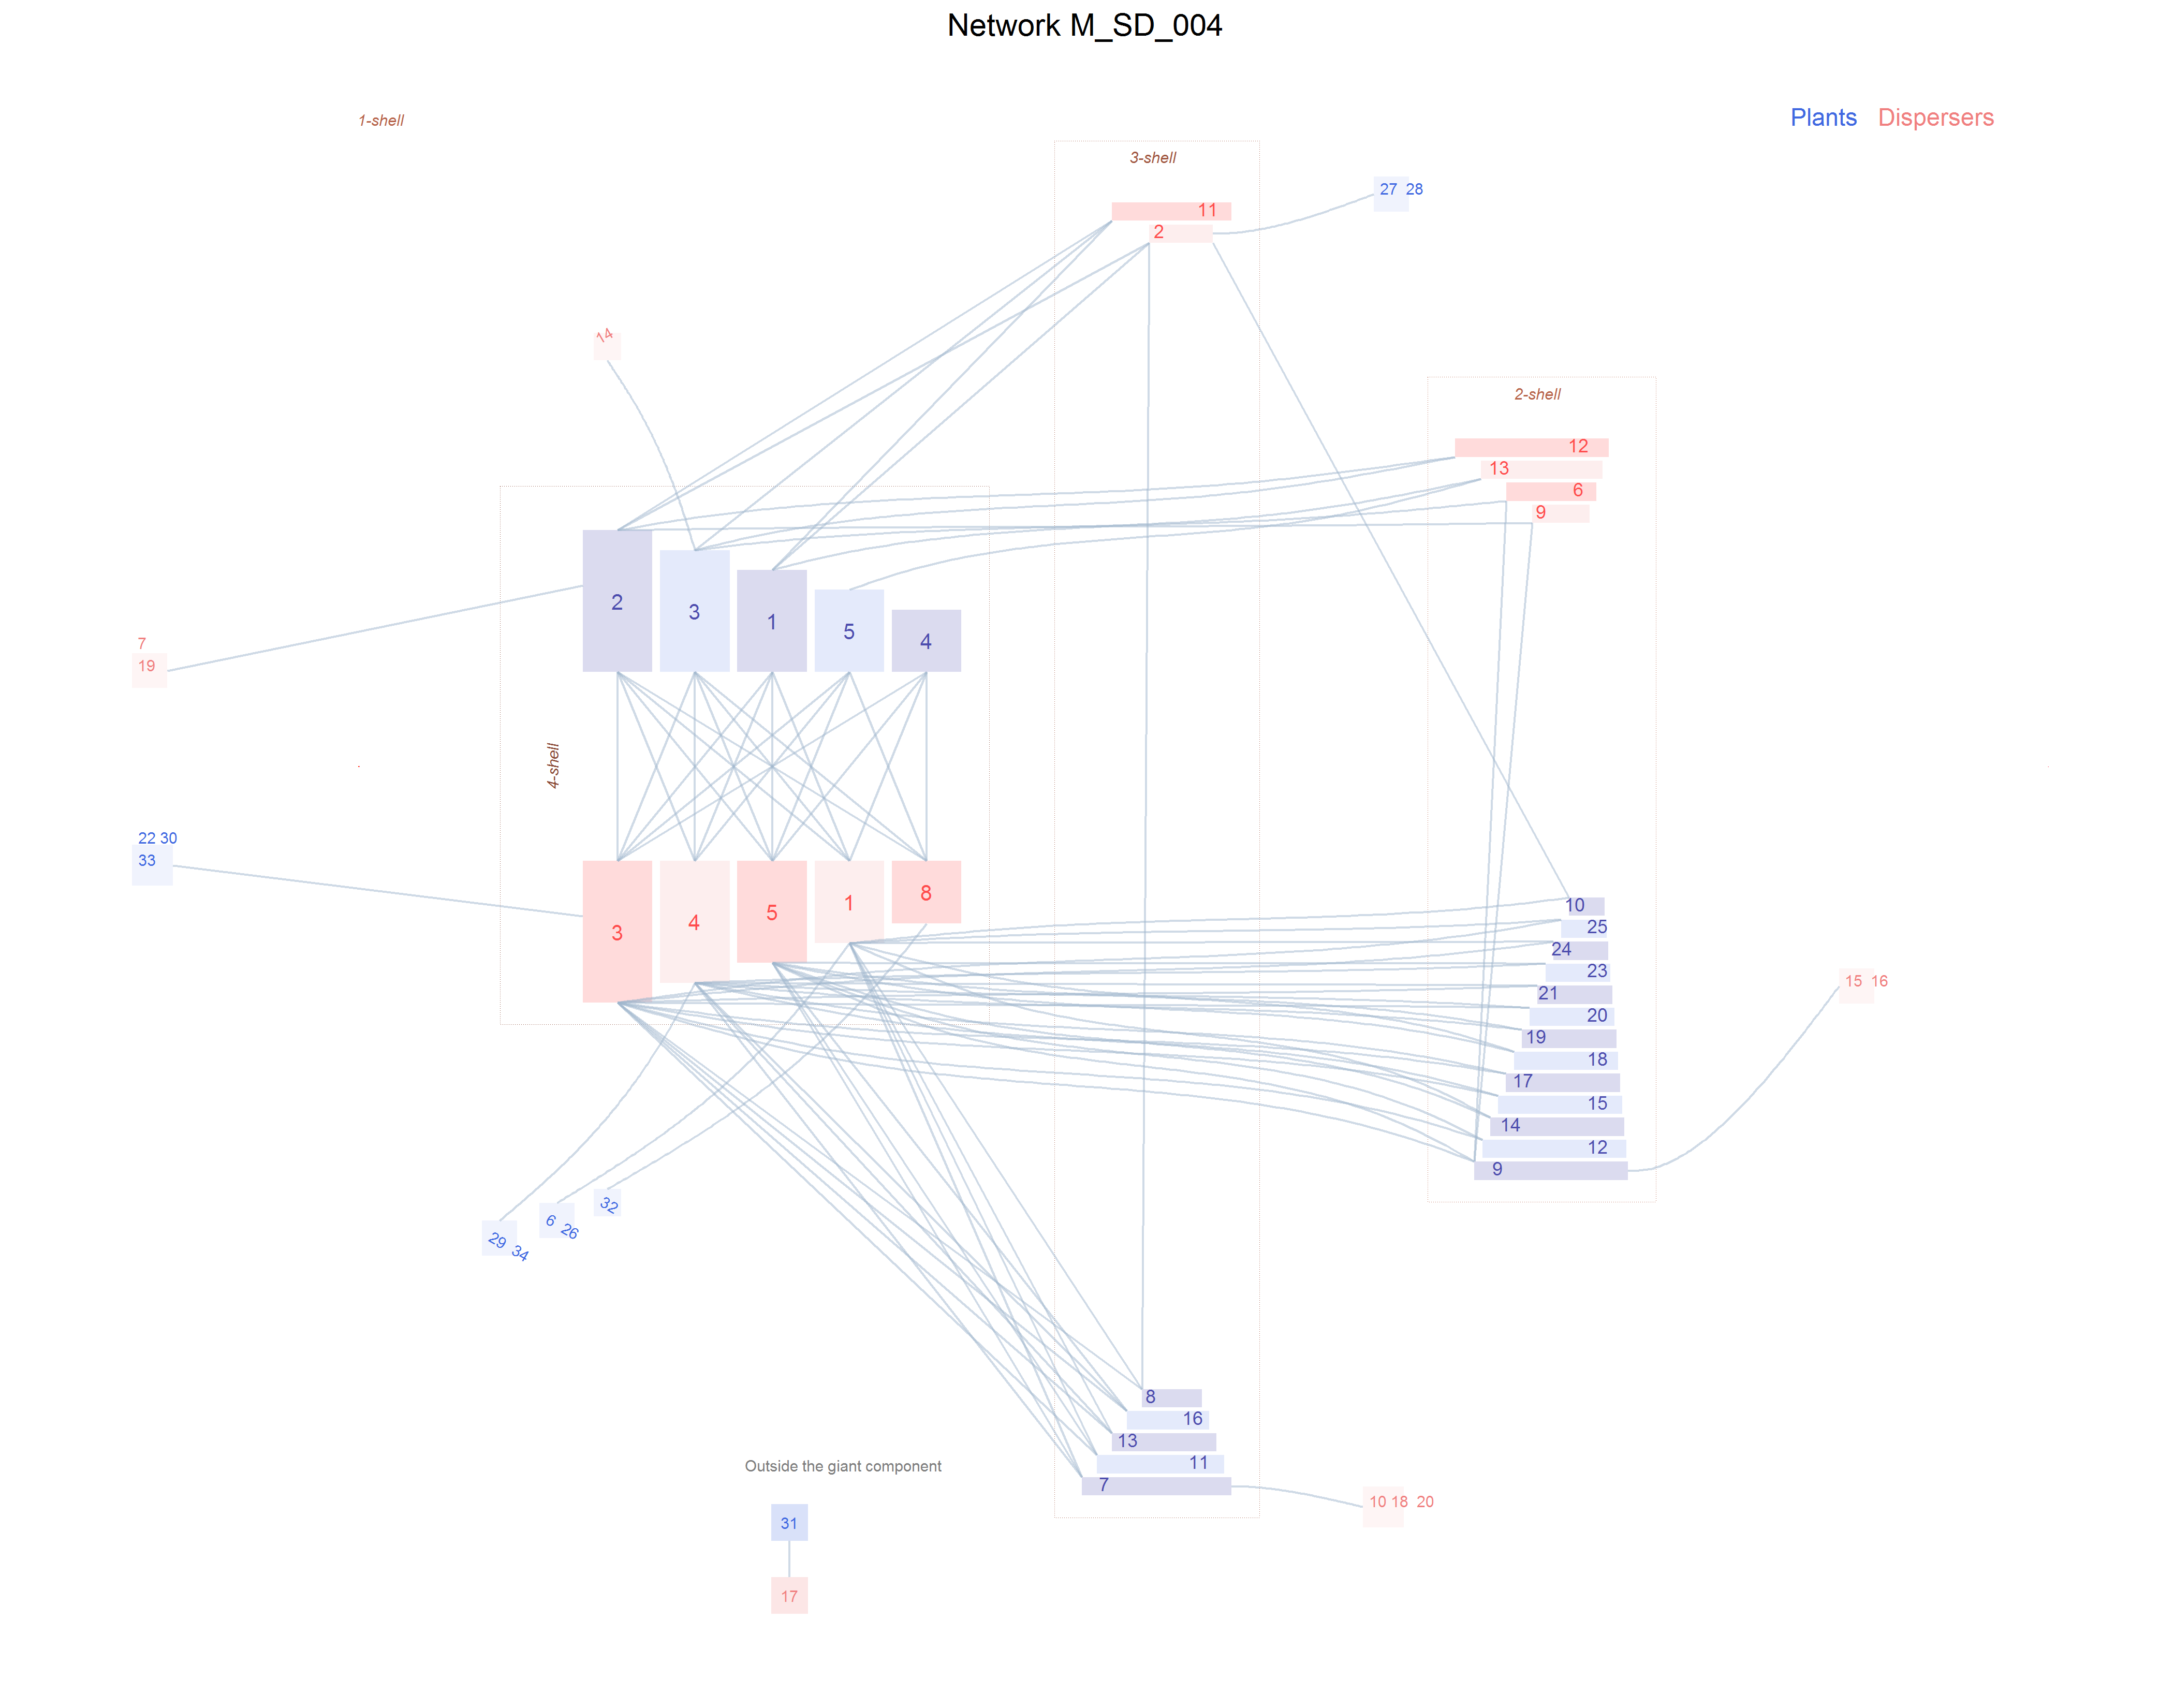
\includegraphics[scale=0.4]{ManFigs/M_SD_004_ziggurat.png}
%\caption {Zigurat de una comunidad de frugívoros en Puerto Rico \cite{carlo2003avian}.}
%\label{fig:AKMAN_ziggurat}
%\end{figure}

Algunos parámetros de entrada son equivalentes a los del  diagrama polar como \texttt{filename}, \texttt{datadir} y \texttt{plotsdir} que 
corresponden al fichero de entrada, al directorio de entrada y al directorio de salida. El fichero de salida se llama
como el de entrada más \texttt{\_ziggurat.png} y el usuario puede también añadir la etiqueta \texttt{file\_name\_append}.

Estos parámetros gráficos proporcionan un conjunto de herramientas muy flexible para mejorar las visualizaciones, como
se puede comprobar en el siguiente ejemplo.

\clearpage
%\fontsize{3.5mm}{3.5mm}\selectfont
%\begin{verbatim}
%ziggurat_graph("data/","M_SD_004.csv",  plotsdir = "grafresults/",
%               height_box_y_expand = 2, factor_hop_x=1.5,
%               color_link = "slategray3", alpha_link = 0.7, 
%               lsize_kcoremax = 6, lsize_zig = 5,lsize_kcore1 = 5,
%               corebox_border_size=0.5, kcore1tail_disttocore = c(1.2,1),
%               displace_outside_component = c(-0.3,1),   
%               lsize_legend = 7, lsize_core_box = 6,
%               displace_legend = c(-0.2,0.2), print_to_file = TRUE)
%\end{verbatim}
%\normalsize
\begin{figure}[hbt!]
\centering
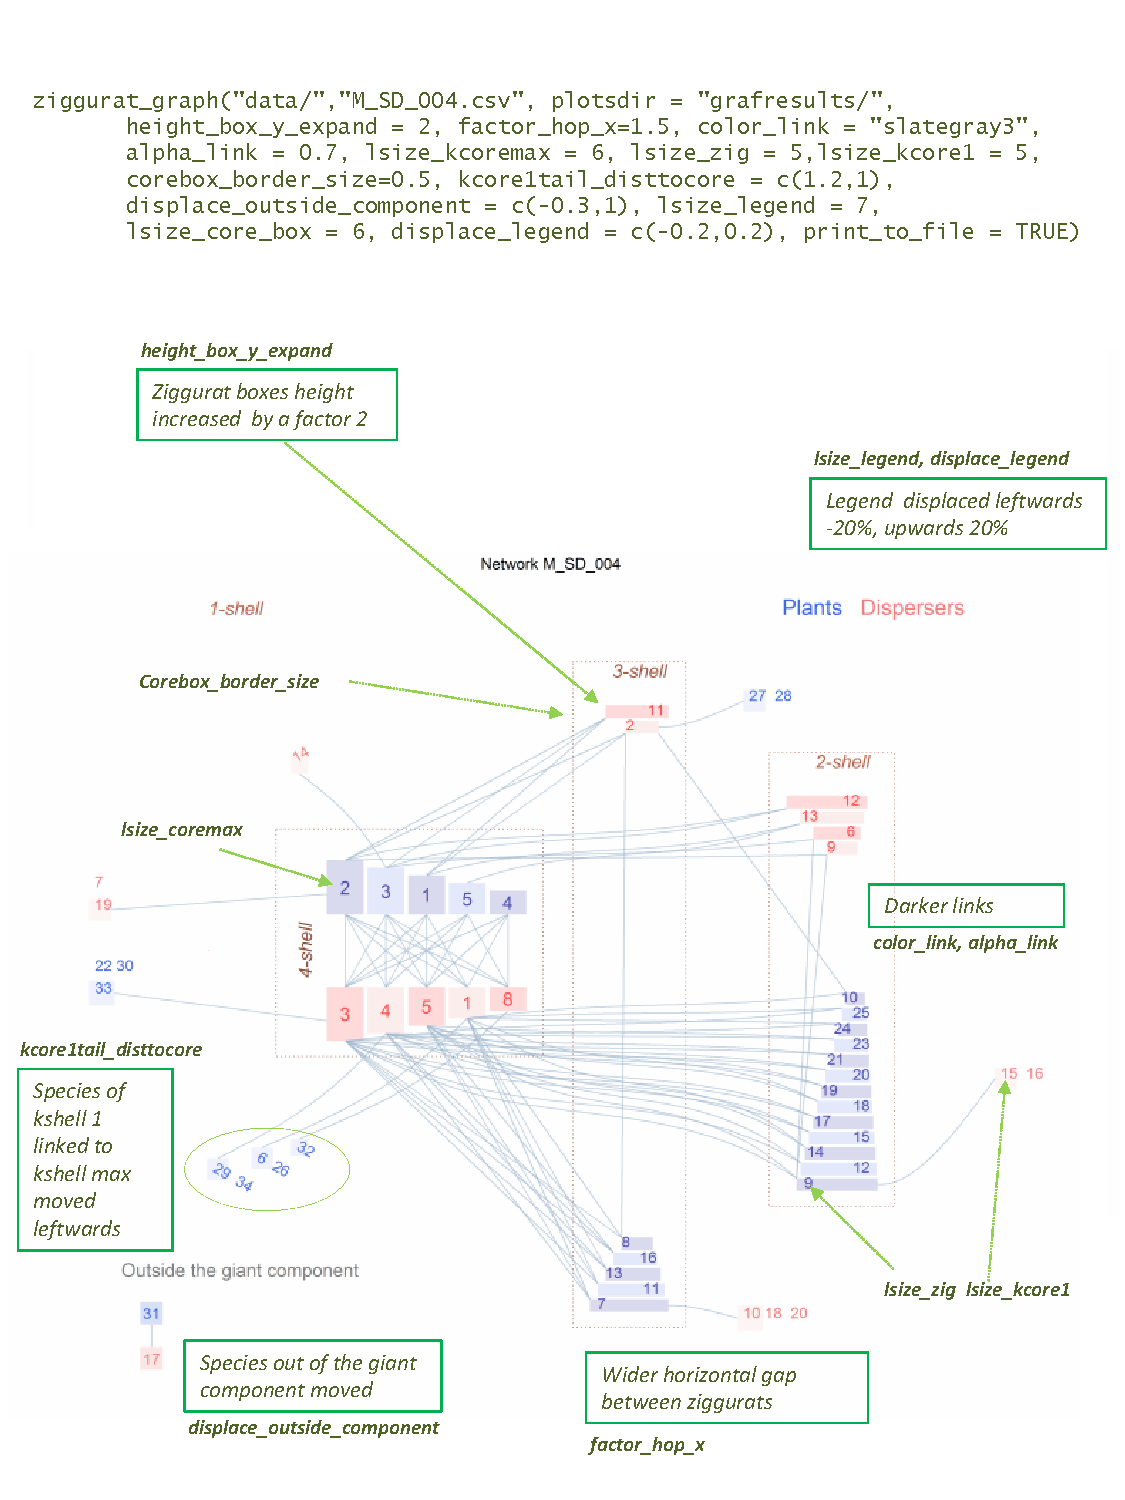
\includegraphics[scale=0.8]{ManFigs/M_SD_004_ziggurat_improved.pdf}
\caption{Zigurat de una comunidad de frugívoros en Puerto Rico \cite{carlo2003avian}.}
\label{fig:M_SD_004_ziggurat_improved}
\end{figure}

\clearpage
La configuración del diagrama puede volverse muy complicada a medida que el tamaño de la red crece. Vamos a demostrar la
utilidad de otro conjunto de parámetros de entrada con una red de tamaño intermedio. La llamada por defecto de la función
proporciona una figura bastante clara de la red de polinizadores número $012$.

\fontsize{3.5mm}{3.5mm}\selectfont
\begin{verbatim}
ziggurat_graph("data/","M_PL_012.csv",  plotsdir = "grafresults/", 
                print_to_file = TRUE)
\end{verbatim}
\normalsize

\begin{figure}[hp!]
\centering
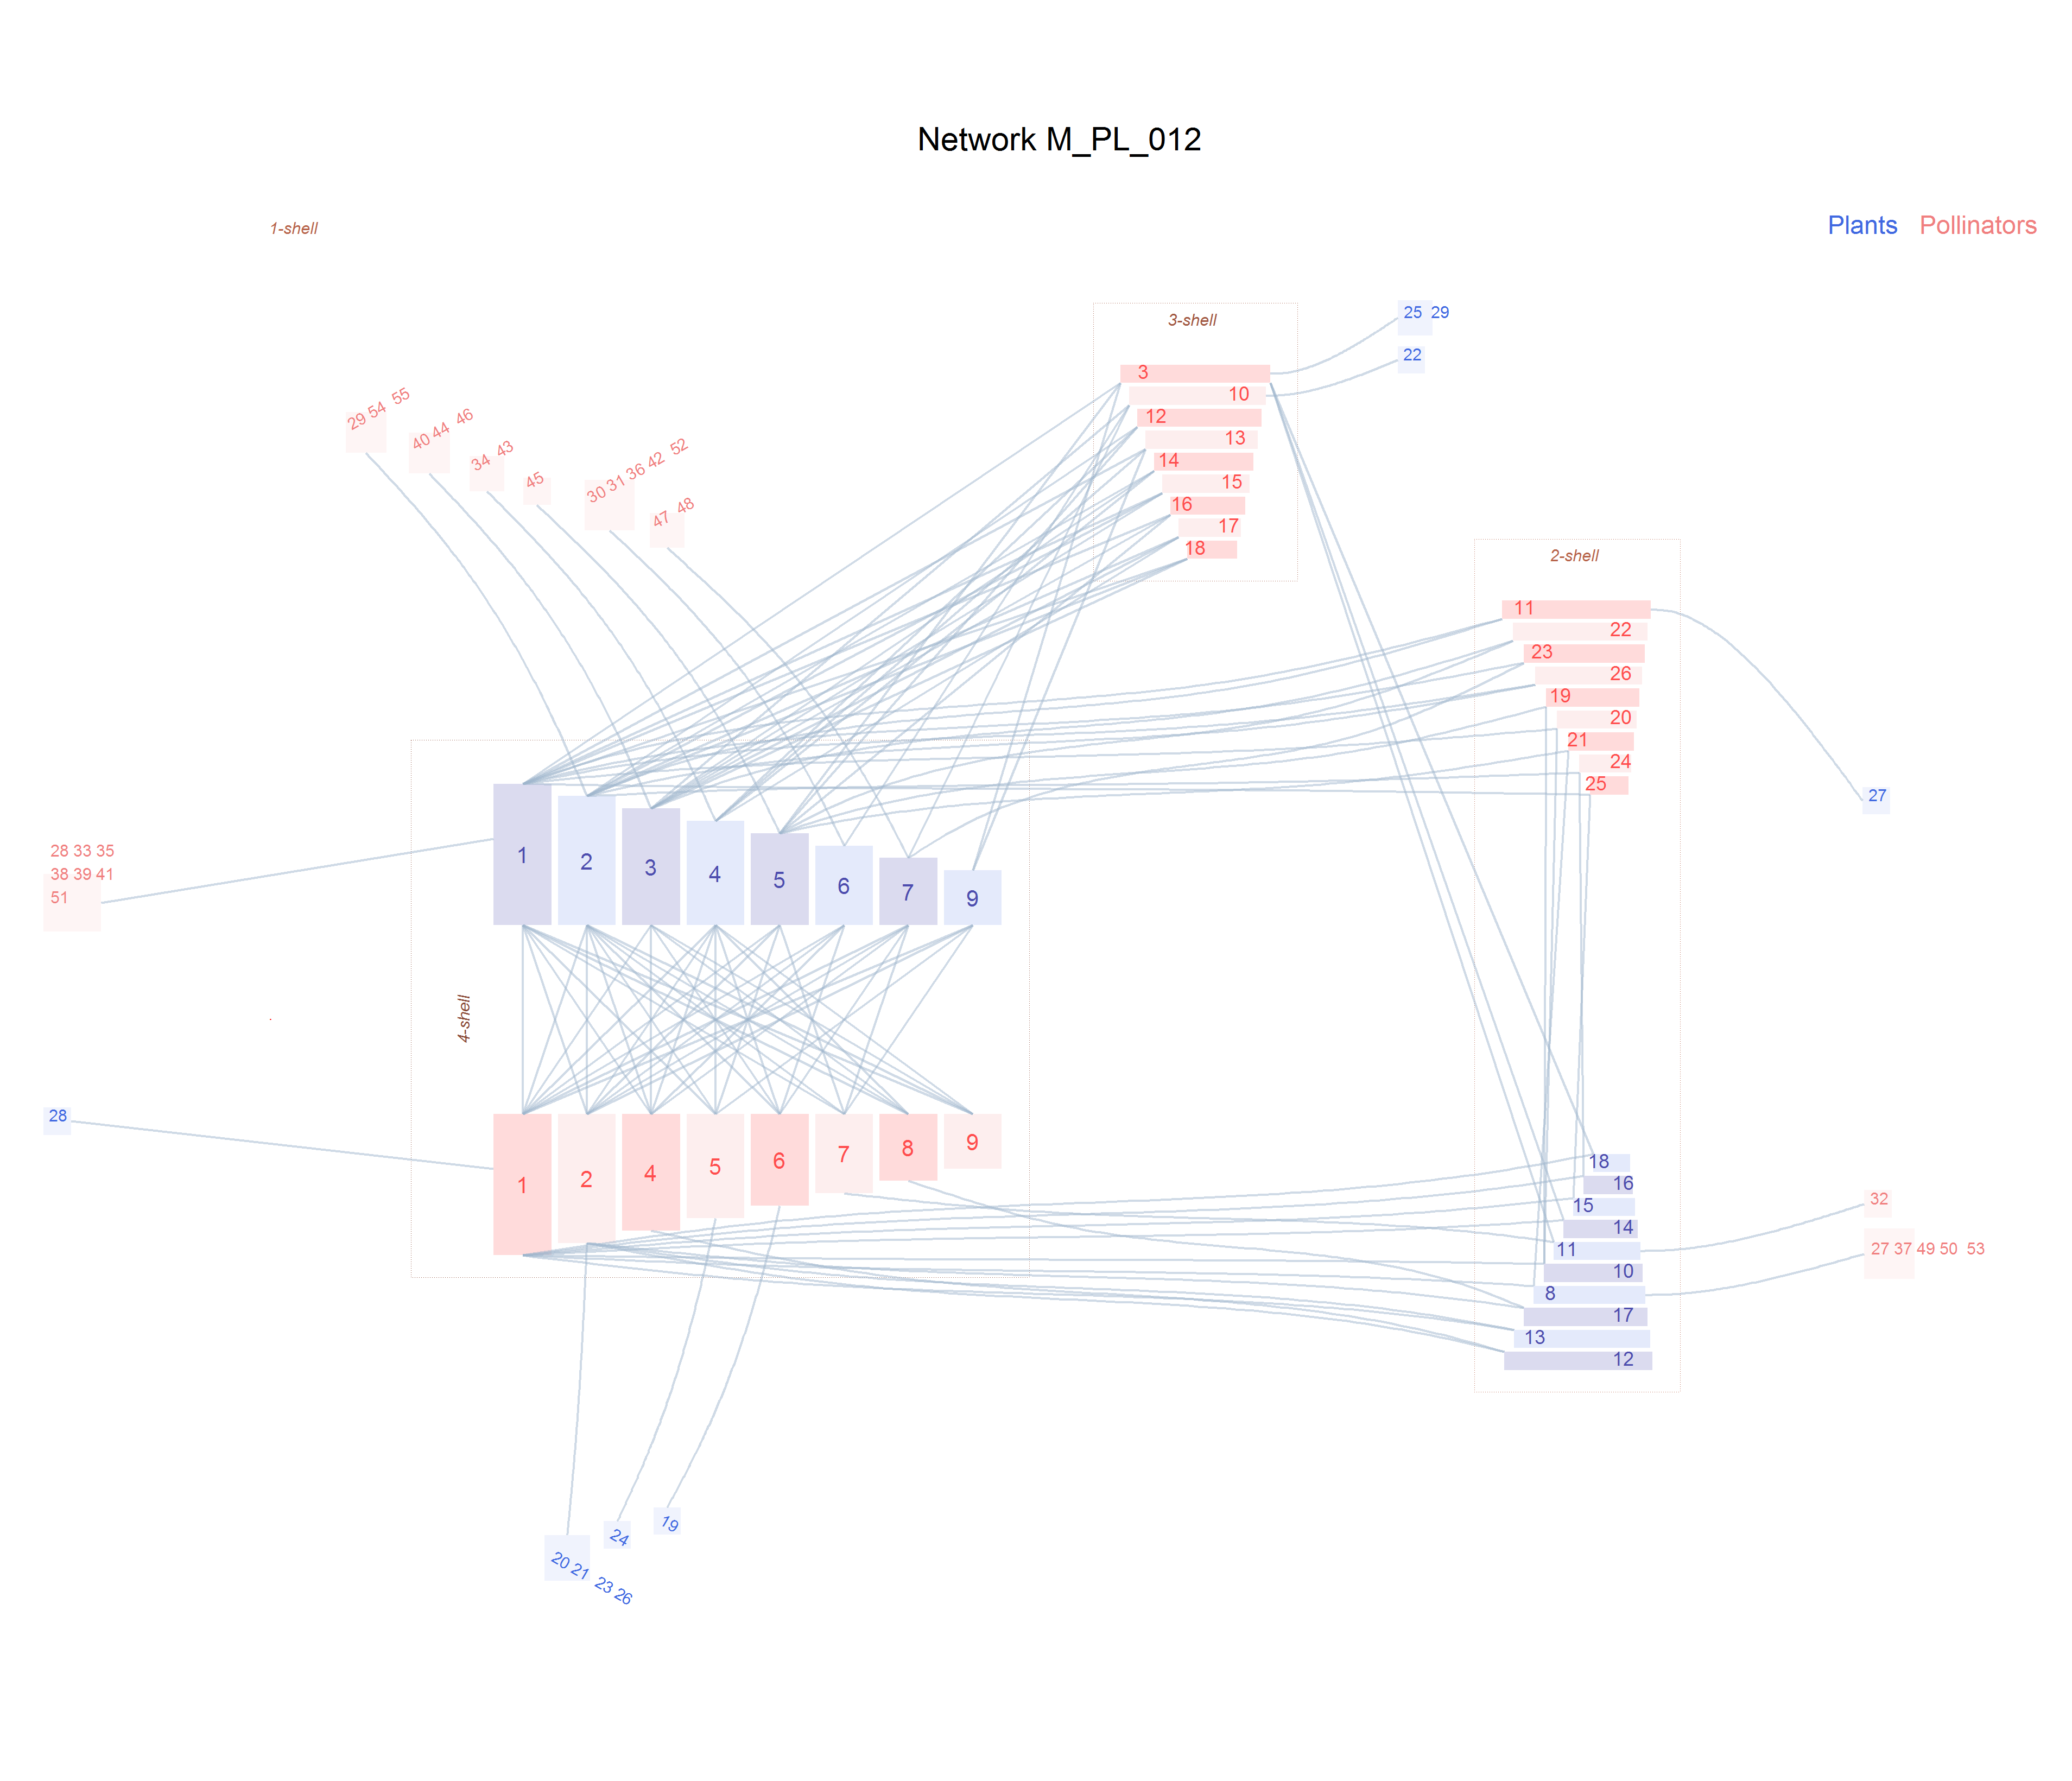
\includegraphics[scale=0.47]{ManFigs/M_PL_012_ziggurat.png}
\caption {Zigurat de una red de polinizadores en el Parque de Garajonay, La Palma (España). Olesen, no publicada.}
\label{fig:AKMAN_ziggurat_012}
\end{figure}

Este gráfico está casi listo para enviar a una publicación, pero hay detalles que podrían mejorarse. Por ejemplo, el tamaño
de las etiquetas que aparecen demasiado pequeñas o la altura de los rectángulos de los zigurats. Vamos a proceder a cambiar 
distintos parámetros de entrada para mostrar como afectan a la imagen.

\clearpage
\begin{figure}[hbt!]
\centering
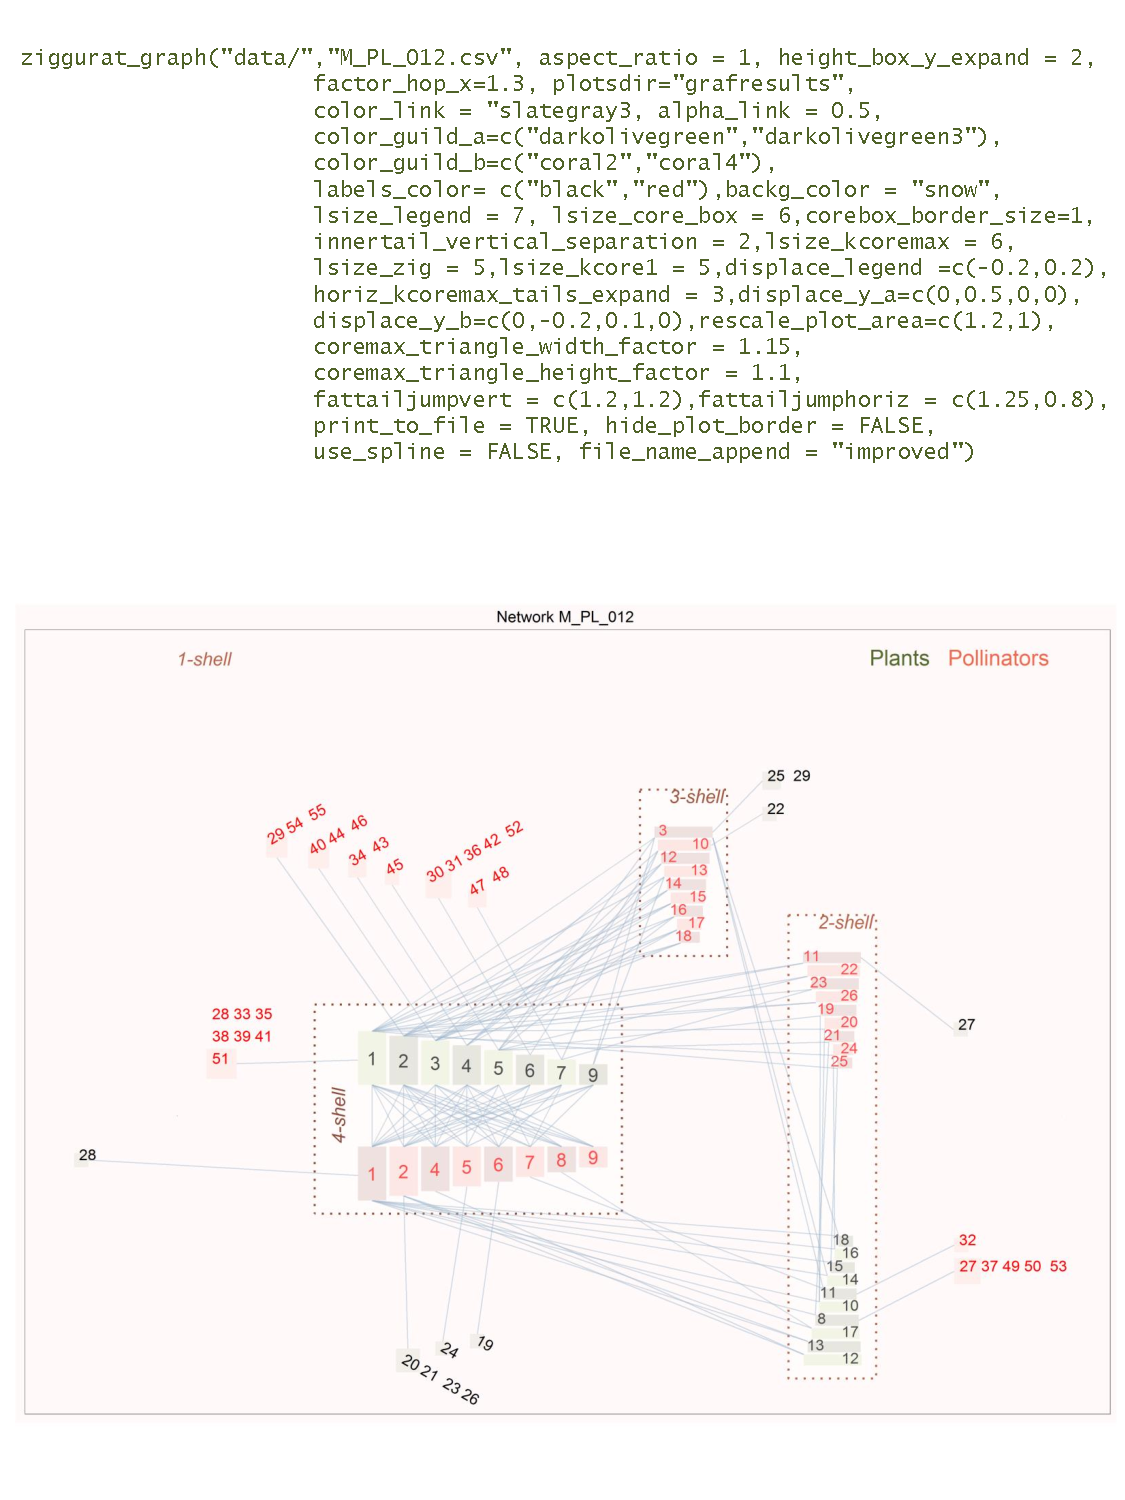
\includegraphics[scale=0.8]{ManFigs/M_PL_012_ziggurat_improved.pdf}
\caption {Ziggurat mejorado de la red $M\_PL\_012$.}
\label{fig:AKMAN_ziggurat_012_improved}
\end{figure}

\clearpage
No vamos a repetir el significado de los que se explicaron en el ejemplo anterior. El papel que desempeñan algunos de los nuevos
es evidente. Se ha cambiado el color de relleno de los zigurats, especificando los pares \texttt{color\_guild\_a} y \texttt{color\_guild\_b},
y también el color de las etiquetas de las especies. Se ha añadido un color de relleno tenue. Este truco sirve para mostrar el área de dibujo, que se ha aumentado en horizontal un $20\%$ con \texttt{rescale\_plot\_area=c(1.2,1)}. Este cambio solo afecta al área de dibujo pero no a la imagen. 

La relación de aspecto puede modificarse para \textit{aplanar} el diagrama si es inferior a $1$ o para \textit{estirarlo} si es mayor. El valor por defecto es $1$, así que no es obligatorio incluirlo en la llamada, pero se ha añadido para explicar su significado.

Si no se usan \textit{splines}, como en este ejemplo, los enlaces aparecen como líneas rectas. Si se usan, se puede indicar cuantos puntos deben tener.

\textit{Fat tails} son los los conjuntos de especies de la \textit{1-shell} que pueden aparecer enlazadas a los generalistas de $k_{degree}$ máximo, los que se encuentran en el extremo izquierdo de la \textit{k-shell} máxima. Se pueden modificar las distancias vertical y horizontal a esas especies con \texttt{fattailjumpvert} y \texttt{fattailjumphoriz}. Obsérvese la posición relativa de la especie de plantas $28$.

Ya vimos como \texttt{height\_box\_y\_expand} controla la altura de las cajas de los zigurats exteriores. La altura y anchura los rectángulos que pertenecen a la \textit{k-shell} máxima de cada clase se modifican con \texttt{coremax\_triangle\_height\_factor} y \texttt{coremax\_triangle\_width\_factor}. 

La distancia horizontal de las especies de la \textit{1-shell} conectadas con la \textit{k-shell} máxima (excepto las \textit{fat tails}) se cambia usando \texttt{horiz\_kcoremax\_tails\_expand}.

La separación vertical entre los zigurats que forman la almendra interior se puede cambiar con los vectores \texttt{displace\_y\_a} y \texttt{displace\_y\_b}. En este diagrama, el zigurat de la \textit{2-shell} de las plantas se mueve hacia arriba un $50\%$, la \textit{2-shell} de los polinizadores hacia abajo un $20\%$ y la \textit{3-shell} de los polinizadores hacia arriba un $10\%$.

Finalmente, la separación vertical de las cadenas conectadas a los zigurats, se puede aumentar con \texttt{innertail\_vertical\_separation}. Véanse las especies de plantas $22$ y $25$.

El siguiente ejemplo muestra como manejar las \textit{weird tails} y los \textit{outsiders}. Las \textit{weird tails} son las cadenas de especies de la \textit{1-shell}. Son muy inestables y por eso no aparecen a menudo. Los \textit{outsiders} son las especies no conectadas a la componente gigante. La red de polinizadores número $031$ contiene especies de ambas clases.

\clearpage
\begin{figure}[hp!]
\centering
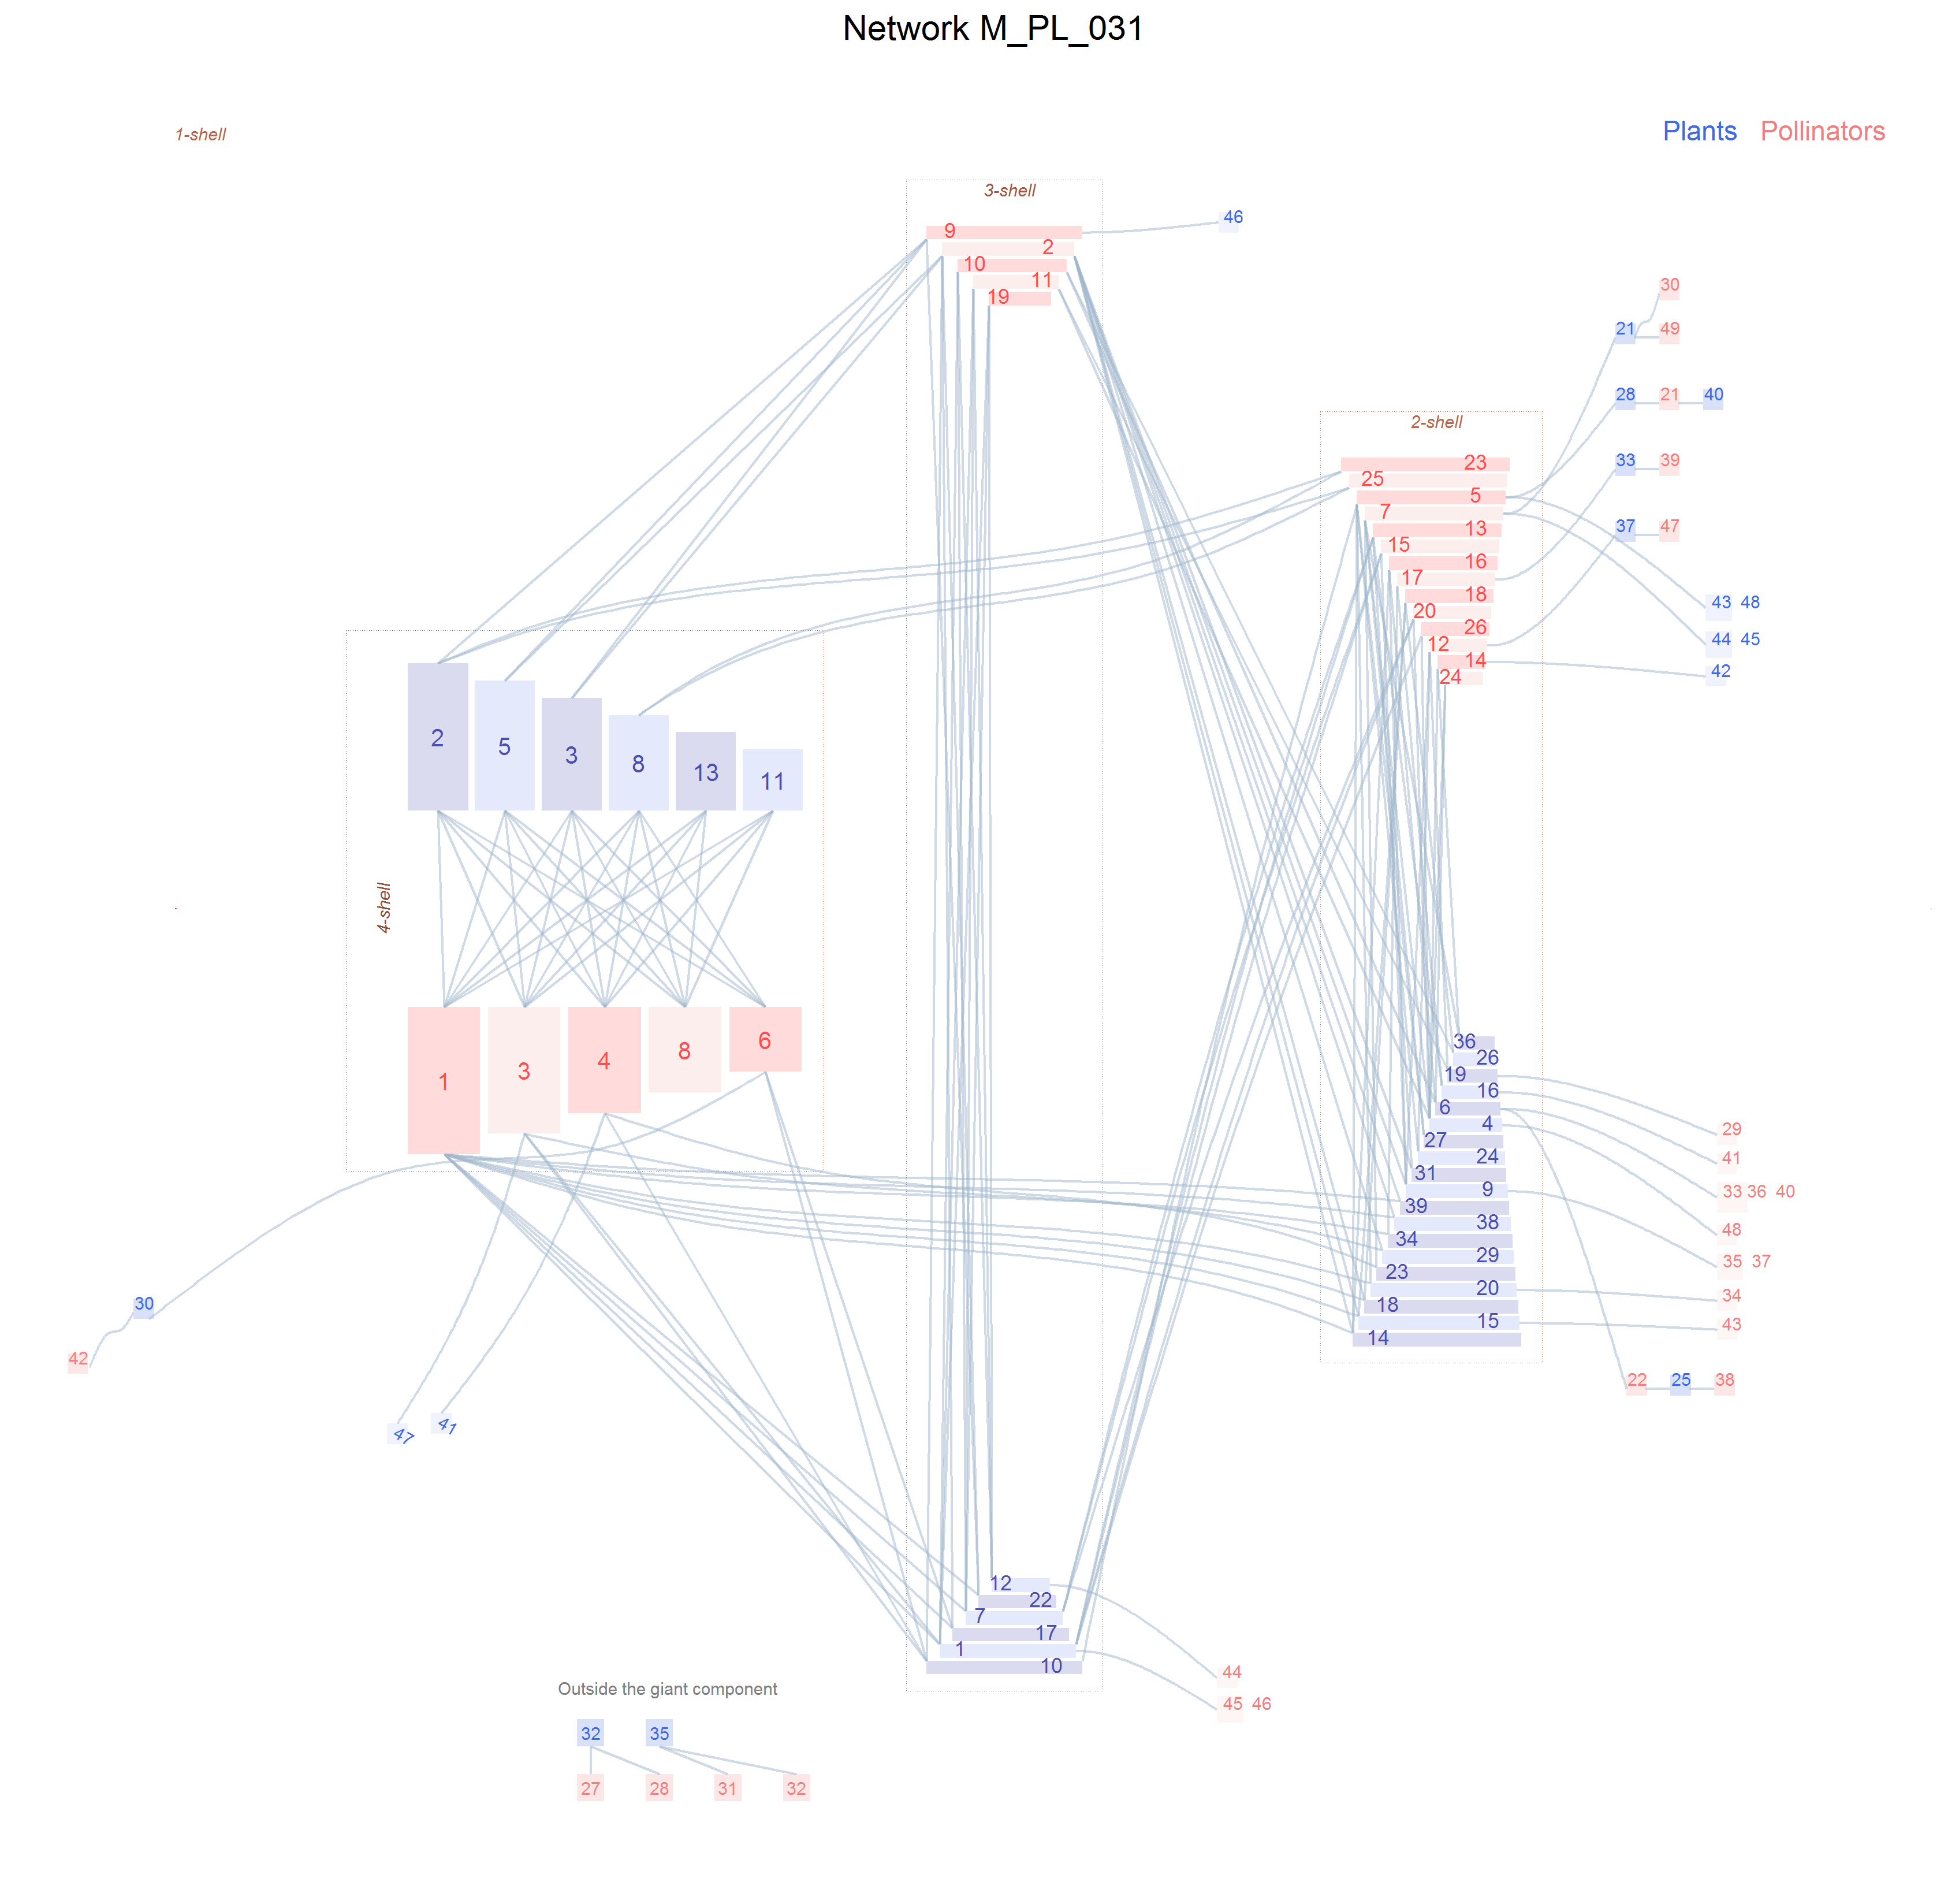
\includegraphics[scale=0.55]{ManFigs/M_PL_031_ziggurat.png}
\caption {Ziggurat de una red de polinizadores en la Alta Guyana (Venezuela) \cite{ramirez1989biologia}.}
\label{fig:AKMAN_ziggurat_031}
\end{figure}

Los \textit{outsiders} aparecen bajo el gráfico principal. Esta red tiene un rico conjunto de \textit{weird chains}, conectadas tanto a los zigurats de la \textit{2-shell} como a la \textit{shell} máxima. Obsérvense las cadenas conectadas a los polinizadores de la \textit{2-shell}, o la formada por la planta $30$ y el polinizador $42$ en el extremo inferior izquierdo.

Si la especie de planta $28$ se extingue, arrastrará al polinizador $21$ y también a la planta $40$. Esta es una rara cadena de especialistas conectadas entre ellas y muy expuesta a las perturbaciones externas. Otra configuración interesante es la formada por la planta $21$ a la que se enlazan los polinizadores $30$ y $49$.

La función \texttt{ziggurat\_graph} ofrece distintos controles de entrada para manejar la apariencia y posición de este tipo de especies.

\clearpage
\begin{figure}[hp!]
\centering
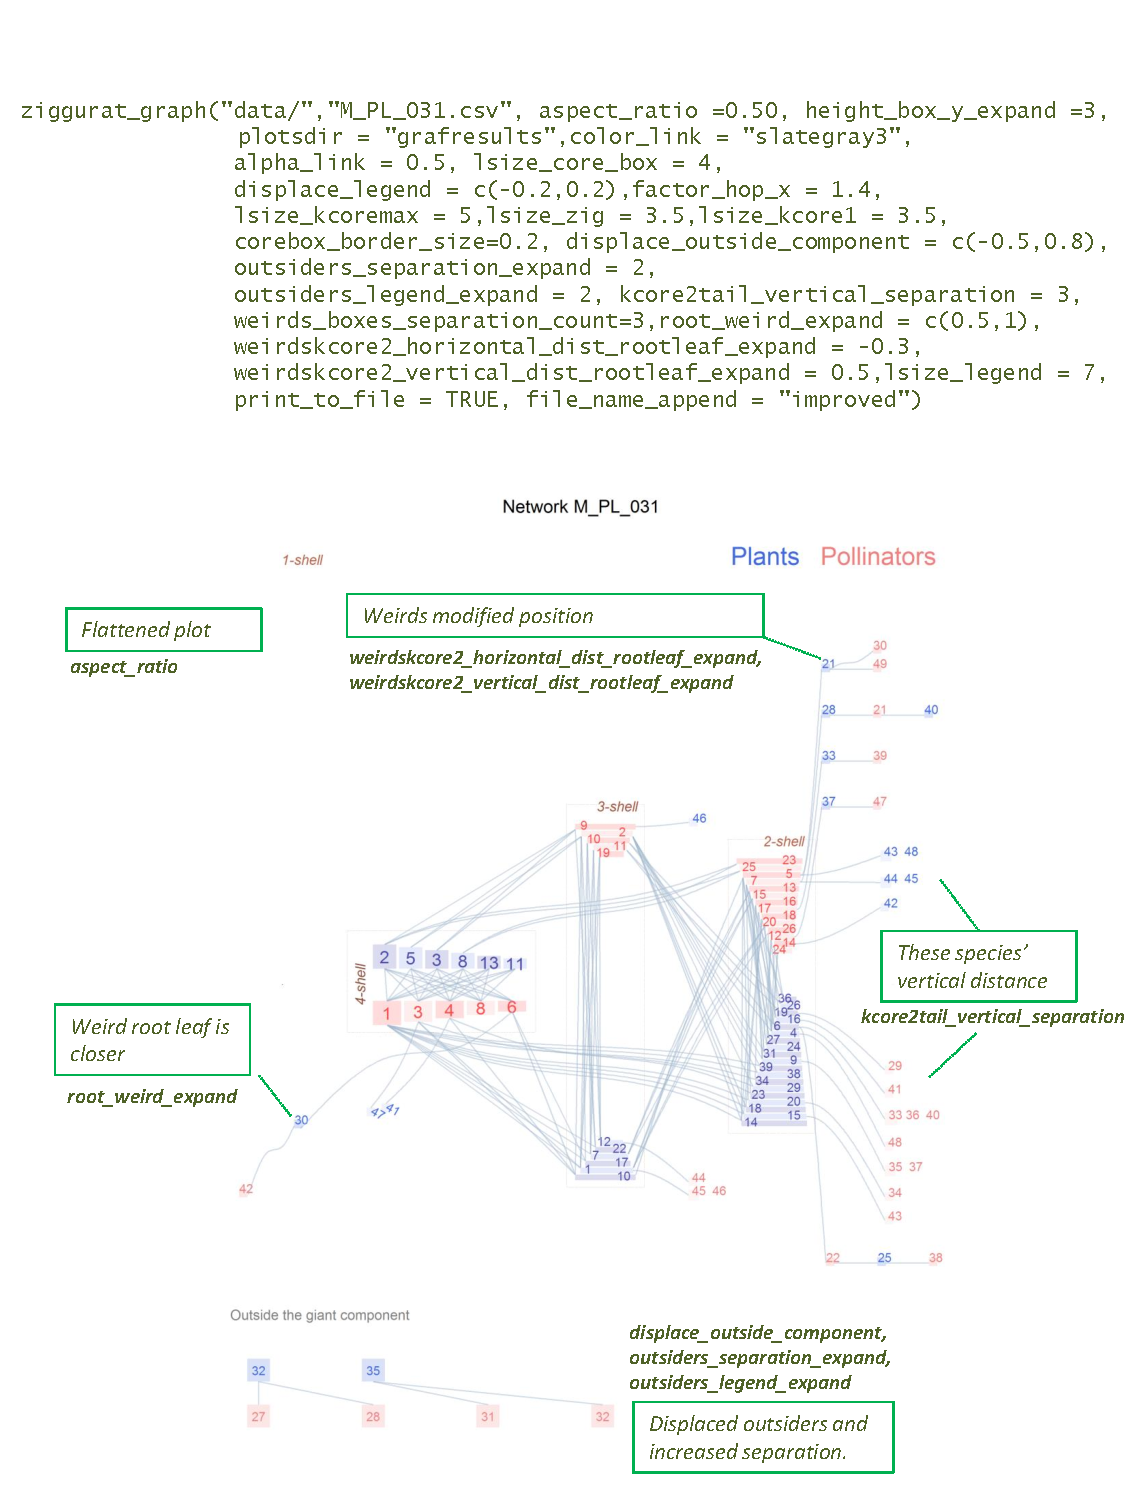
\includegraphics[scale=0.8]{ManFigs/M_PL_031_ziggurat_improved.pdf}
\caption {Zigurat mejorado de la figura \ref{fig:AKMAN_ziggurat_031}.}
\label{fig:AKMAN_ziggurat_031}
\end{figure}


\clearpage
Es posible mostrar los nombres de las especies dentro de los rectángulos. Puesto que los nombres científicos suelen ser largos, conviene abreviarlos quedándose solo con los $n$ primeros caracteres de ambos elementos de la nomenclatura binomial. Esto se consigue con el parámetro \texttt{shorten\_species\_name}. Como se ha indicado al hablar de las etiquetas de especie en el diagrama polar, hay que tener cuidado, porque pueden convertir en ilegible el diagrama. No se recomienda su uso si no es para redes pequeñas. En ningún caso se muestran los nombres de las especies de la \textit{1-shell}.

\begin{figure}[hp!]
\centering
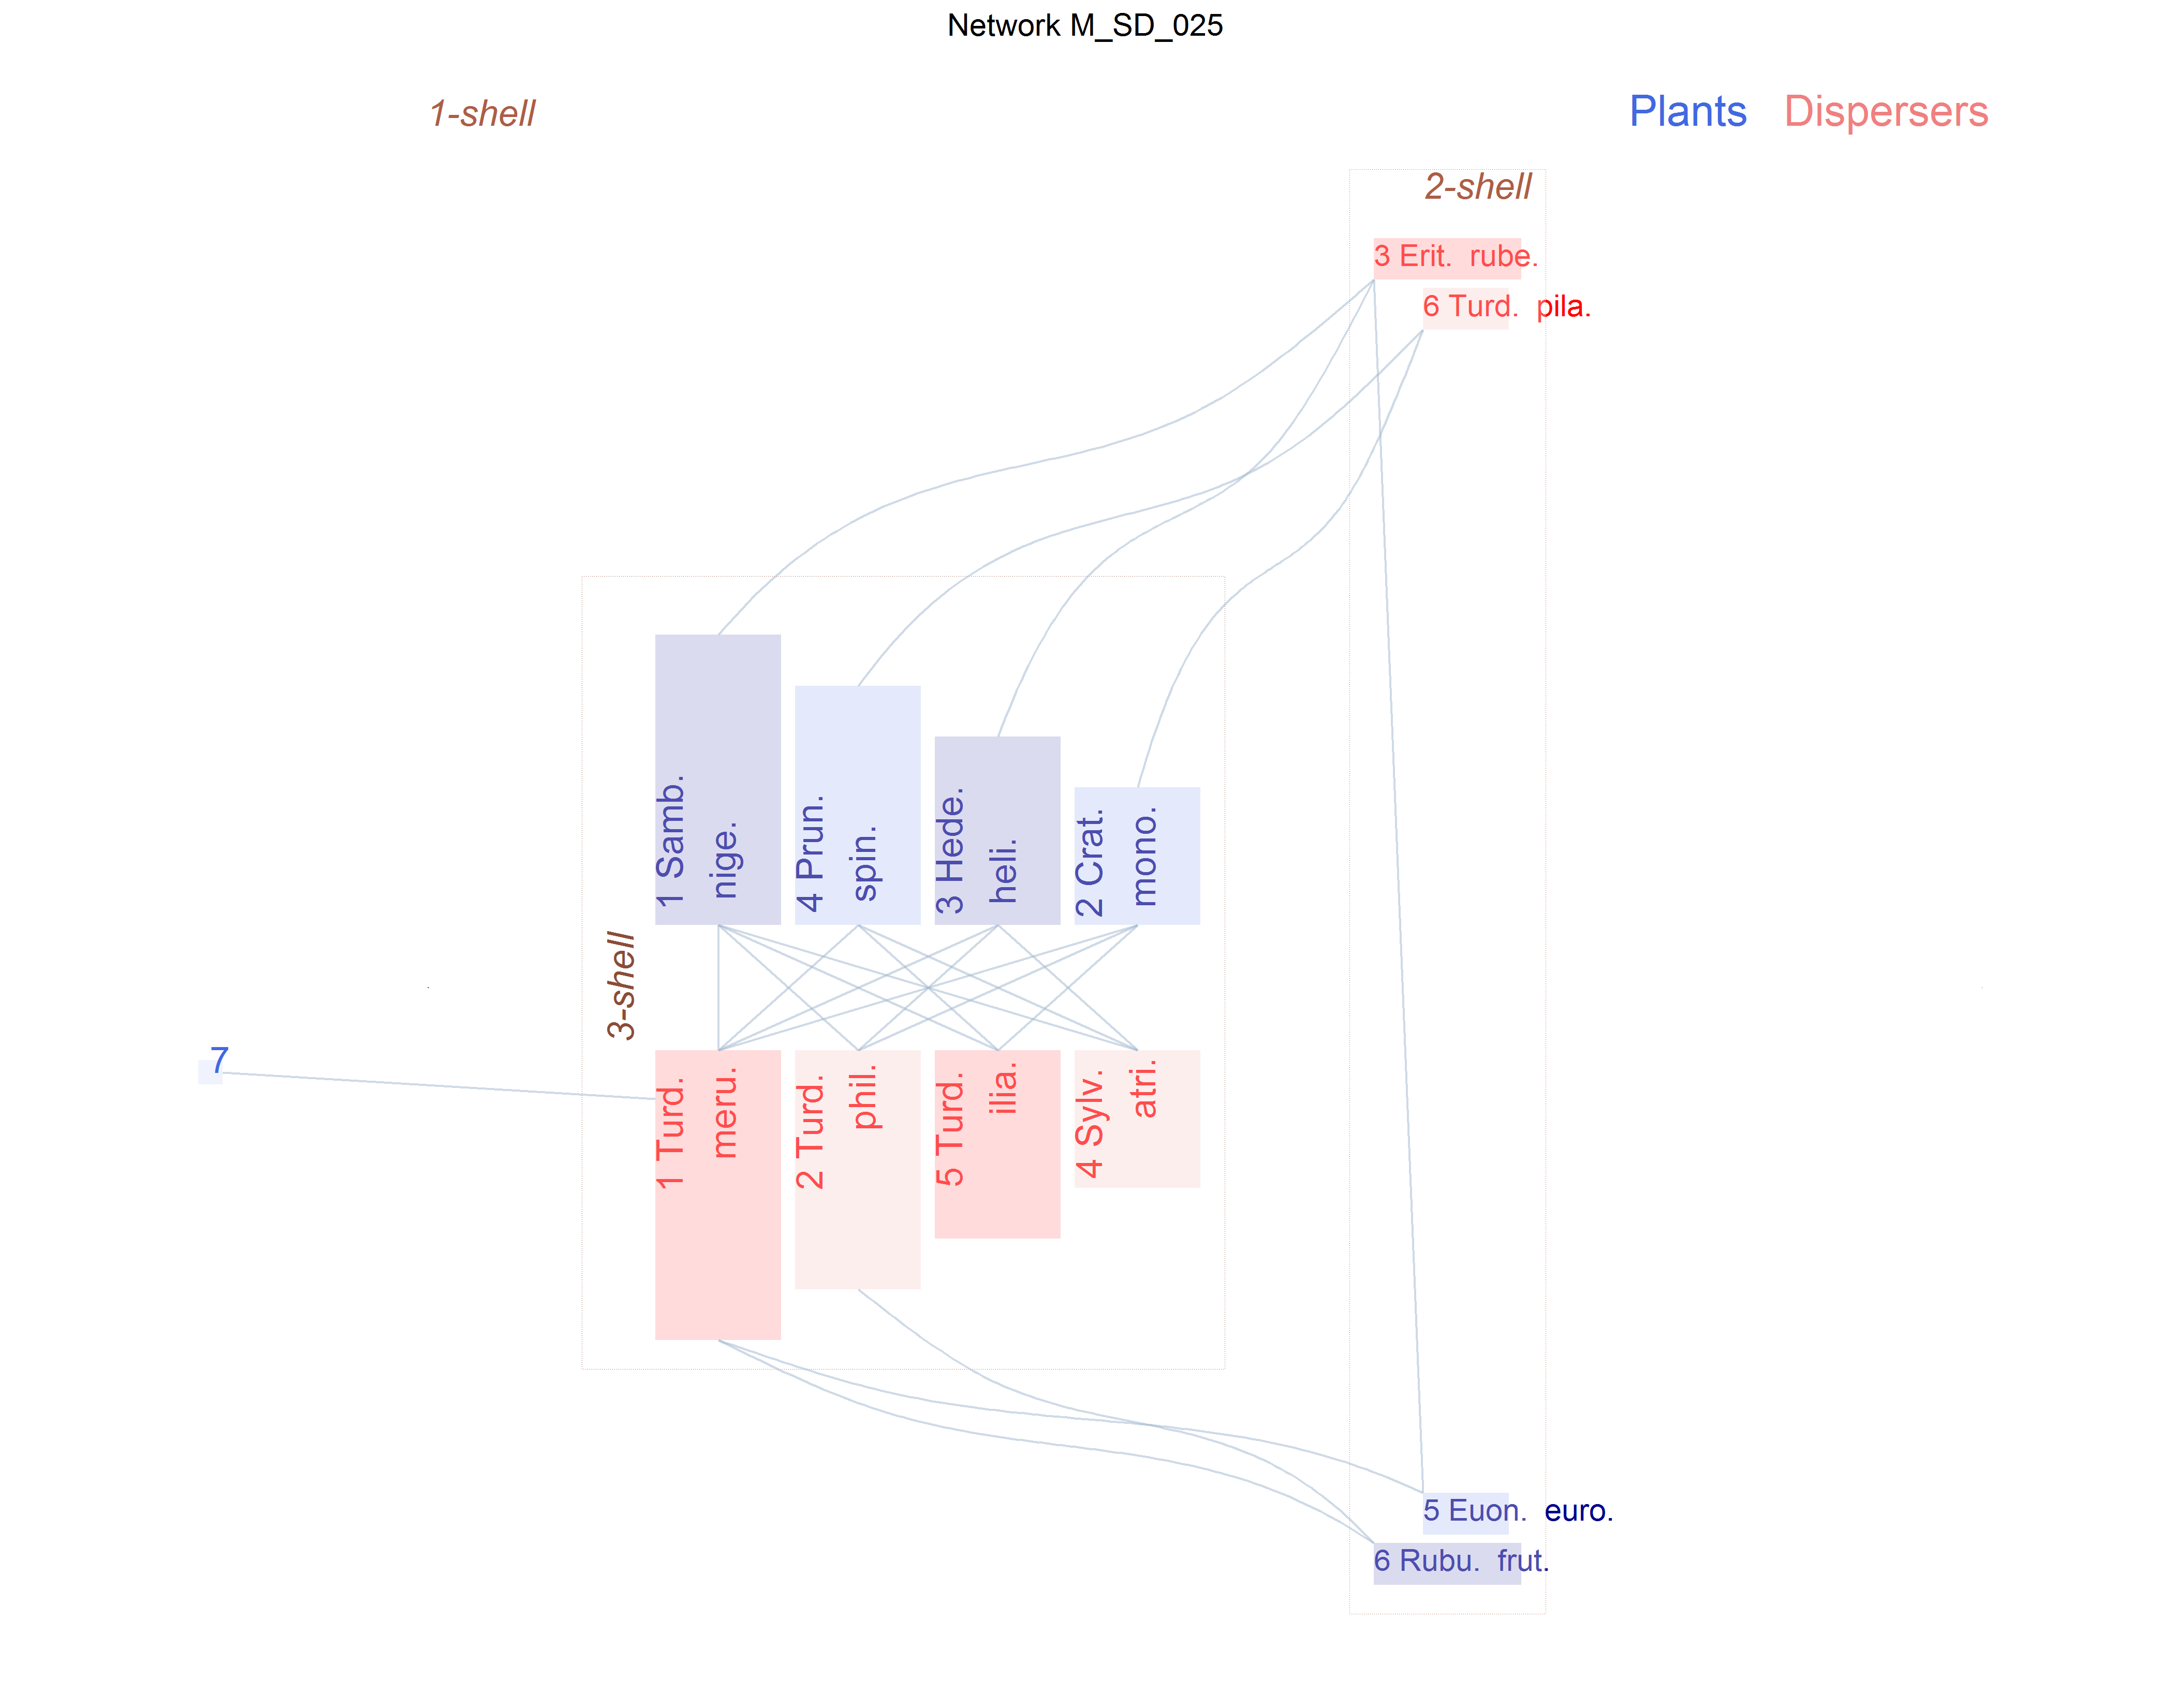
\includegraphics[scale=0.48]{ManFigs/M_SD_025_ziggurat.png}
\caption {Zigurat con nombres de especies.}
\label{fig:AKMAN_ziggurat_025}
\end{figure}

\fontsize{3.5mm}{3.5mm}\selectfont
\begin{verbatim}
ziggurat_graph("./data/","M_SD_025.csv",plotsdir="grafresults/",
               shorten_species_name = 4, displace_legend = c(-0.2,0.2),
               height_box_y_expand = 2, coremax_triangle_width_factor = 1.25,
               coremax_triangle_height_factor = 2.25,lsize_core_box = 6,
               lsize_kcoremax = 6, lsize_legend= 7,lsize_kcore1 = 6, 
               lsize_zig = 5, kcore_species_name_display = c(2,3), 
               kcore_species_name_break = c(3), print_to_file = TRUE)

\end{verbatim}
\normalsize

\clearpage
\noindent La función devuelve su propio entorno llamado \texttt{zgg} donde se almacenan los parámetros de configuración y los resultados. Usándolo puede consultarse:

\begin{itemize}

\item \texttt{zgg\$plot}:  el diagrama zigurat.

\item \texttt{zgg\$svg}: el diagrama como objeto SVG.

\item \texttt{zgg\$results\_analysis}: resultados de la llamada interna a \texttt{analyze\_network}.

\end{itemize}
 

\noindent Por último, este es el significado de los parámetros de entrada:
\small
\begin{itemize}

\item \texttt{datadir}:  directorio donde está el fichero de la matriz.

\item \texttt{filename}: nombre del fichero de la matriz.

\item \texttt{print\_to\_file}: si se indica FALSE el diagrama se representa en la ventana de la sesión R.

\item \texttt{plotsdir}: directorio de salida.

\item \texttt{flip\_results}: gira el gráfico 90 grados.

\item \texttt{aspect\_ratio}: relación de aspecto.

\item \texttt{alpha\_level}: transparencia en el relleno de los zigurats.

\item \texttt{color\_guild\_a}: relleno por defecto de las especies de la clase a.

\item \texttt{color\_guild\_b}: relleno por defecto de las especies de la clase b.

\item \texttt{color\_link default}: color de los enlaces.

\item \texttt{alpha\_link}: transparencia de los enlaces.

\item \texttt{size\_link}: anchura de los enlaces.

\item \texttt{displace\_y\_b}: desplazamiento vertical relativo de los zigurats de la clase b.

\item \texttt{displace\_y\_a}: desplazamiento vertical relativo de los zigurats de la clase a.

\item \texttt{labels\_size}: tamaño de las etiquetas.

\item \texttt{lsize\_kcoremax}: etiquetas de la kshell máxima.

\item \texttt{lsize\_zig nodes}: etiquetas de los nodos de los zigurats.

\item \texttt{lsize\_kcore1}: etiquetas de los nodos de kshell 1.

\item \texttt{lsize\_legend}: etiquetas de la leyenda de clases.

\item \texttt{lsize\_kcorebox}: etiquetas de las cajas que rodean las kshells.

\item \texttt{labels\_color}: color de las etiquetas.

\item \texttt{height\_box\_y\_expand}: multiplicar la altura de los rectángulos de zigurat por este factor.

\item \texttt{kcore2tail\_vertical\_separation}: modifica la distancia vertical de los nodos de kshell 1 conectados a kshell 2.

\item \texttt{kcore1tail\_disttocore}:  modifica la distancia vertical de los nodos de kshell 1 conectados a las kshell max (guild\_a, guild,b).

\item \texttt{innertail\_vertical\_separation}: modifica la distancia vertical de los nodos de kshell 1 conectados a $2 < kshell < kshell max$.

\item \texttt{horiz\_kcoremax\_tails\_expand}: modifica la distancia horizontal de las weird tails conectadas a kshell max.

\item \texttt{factor\_hop\_x expand inner}: modifica la separación horizontal de los zigurats.

\item \texttt{displace\_legend modify}: modifica la posición de la leyenda de clases.

\item \texttt{fattailjumphoriz}: desplaza las fat tails horizontalmente.

\item \texttt{fattailjumpvert}: desplaza las fat tails verticalmente.

\item \texttt{coremax\_triangle\_width\_factor}: expande la anchura de los rectángulos de la kshell max.

\item \texttt{coremax\_triangle\_height\_factor}: expande la altura de los rectángulos de la kshell max.

\item \texttt{paint\_outsiders}: muestra los outsiders.

\item \texttt{displace\_outside\_component}: desplaza los outsiders (horizontal, vertical).

\item \texttt{outsiders\_separation\_expand}: multiplica la separación de los outsiders.

\item \texttt{outsiders\_legend\_expand}: desplaza la leyenda de outsiders.

\item \texttt{weirdskcore2\_horizontal\_dist\_rootleaf\_expand}: expande la distancia horizontal del nodo raíz de una weird tail conectada a kshell 2.

\item \texttt{weirdskcore2\_vertical\_dist\_rootleaf\_expand}: expande la distancia vertical del nodo raíz de una weird tail conectada a kshell 2.

\item \texttt{weirds\_boxes\_separation\_count}: número de cajas de separación de las especies de las weird tails.

\item \texttt{root\_weird\_expand}: multiplica la distancia del nodo raíz de una weird tail conectada a kshell != 2.

\item \texttt{hide\_plot\_border}: oculta el borde del gráfico.

\item \texttt{rescale\_plot\_area}: cambiar el tamaño del área de dibujo (horizontal, vertical).

\item \texttt{kcore1weirds\_leafs\_vertical\_separation}: mutiplica la separación vertical de las weird tails conectadas a kshell 1.

\item \texttt{corebox\_border\_size}: anchura de la línea de las cajas que rodean las kshells.

\item \texttt{kcore\_species\_name\_display}: muestra los nombres de las especies de las kshells incluidas en este vector.

\item \texttt{kcore\_species\_name\_break}: permite saltos de línea en los nombres de las especies de las kshells incluidas en este vector.

\item \texttt{shorten\_species\_names}: número de caracteres de los nombres de especies que se muestran.

\item \texttt{label\_strguilda}: etiquetas de la clase a.

\item \texttt{label\_strguildb}: etiquetas de la clase b.

\item \texttt{landscape\_plot}: configuración del papel en modo horizontal.

\item \texttt{backg\_color}: relleno de fondo.

\item \texttt{show\_title}: mostrar el título del gráfico.

\item \texttt{use\_spline}: usar splines para dibujar los enlaces.

\item \texttt{spline\_points}: número de puntos de los splines.

\item \texttt{file\_name\_append}: etiqueta que el usuario puede añadir al fichero de salida.

\item \texttt{svg\_scale\_factor}: solo para aplicaciones interactivas, no modificar.

\item \texttt{progress}: solo para aplicaciones interactivas, no modificar.
\end{itemize}
